\documentclass[a4paper]{article}

\usepackage[utf8]{inputenc}
\usepackage[T1]{fontenc}
\usepackage{textcomp}
\usepackage[dutch]{babel}
\usepackage{amsmath, amssymb}
\usepackage{code}
\usepackage{pythonhighlight}

% figure support
\usepackage{import}
\usepackage{xifthen}
\pdfminorversion=7
\usepackage{pdfpages}
\usepackage{transparent}
\usepackage{float,graphicx}
\pdfsuppresswarningpagegroup=1
\graphicspath{{./img/}}

\begin{document}
   \section{Overview} 
   \begin{itemize}
       \item taxanomy
       \item MR path planning 
           \begin{itemize}
               \item Discrete
               \item continous
           \end{itemize}
        \item Concurrent assignment and path planning 
   \end{itemize}
   \section{Taxanomy}
   \begin{itemize}
       \item Domain : continous and Discrete 
           \begin{itemize}
               \item continous planning time parameterised trajecteroies
               \item planning on graphs or grids
           \end{itemize}
       \item Goal assignment 
           \begin{itemize}
               \item \textbf{Labeled} each robot has pre determined goal 
               \item \textbf{Inlabeled} no pre determined path but goal must be reached
           \end{itemize}
       \item problem representation
           \begin{itemize}
               \item \textbf{coupled} joint state of all robots in the system
               \item \textbf{Decoupled} each robot is represented individually
           \end{itemize}
       \item planning
           \begin{itemize}
               \item \textbf{Reactive} dynamic obstacle avoidance
               \item \textbf{Deliberative} optimilaty 
           \end{itemize}
        \item Computation
            \begin{itemize}
                \item \textbf{Centralised}
                \item \textbf{Decentralised}
            \end{itemize}
   \end{itemize}
   \section{Multi agent path planning}
   \begin{itemize}
       \item Multi agent path planning is also called as multi agent path planning
       \item discretized robot
       \item point robots - holonomic and no motion constrains
   \end{itemize}
   \subsection{The problem}
   \begin{itemize}
       \item no of agents at start location with predefined goal in known environment
       \item \textbf{Task} find a collsion free path
   \begin{itemize}
       \item generally this is an Labeled problem
       \item \textbf{application} logistics,automated warehouse
   \end{itemize}
        \item \textbf{allowed motion} - north,south,east,west
    \end{itemize}
    \subsubsection{Performance metrics}
    \begin{itemize}
        \item \textbf{Makespan} - time of last robots arrival 
        \item \textbf{Flowtime} - sum of arrival time, over all robots
    \end{itemize}
    \section{Coupled vs decoupled}
    \begin{figure}[htpb]
                       \centering
                       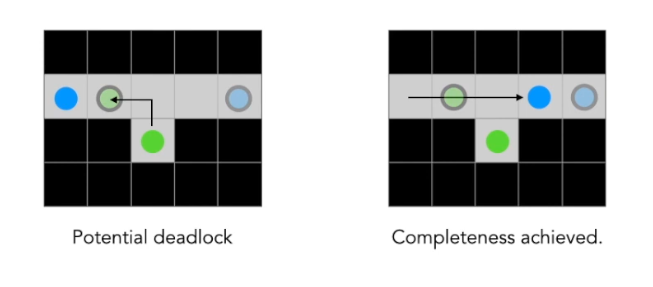
\includegraphics[width=0.8\textwidth]{cvdpathplanning.png}
                       \caption{}
                       \label{fig:}
                   \end{figure}
    \begin{itemize}
        \item coupled planning gives completeness
        \item Decoupled path planning is not complete in general(prone to Deadlock)
    \end{itemize}
    \section{Coupled path planning}
    \begin{itemize}
        \item Complexity over decoupled
        \item but more power solution
        \item coupled formulation:
            \begin{itemize}
                \item Robot $i$ has configuration space \footnote{a complete specification of the position of every point in the system} of  $C_i$
                \item Then joint state is given by product:\\
                        $X=C_1*C_2*C_3*C_4 \ldots\ldots$
                \item dimensionality grows linearly
                \item A* requires time that is exponential to space
            \end{itemize}
        \item for $N$ robots in  $M$ cells in grid world 
        \begin{figure}[H]
                \centering
                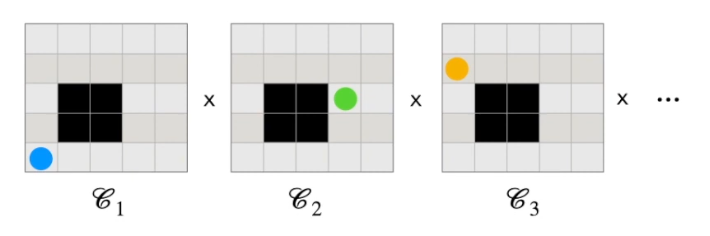
\includegraphics[width=0.8\textwidth]{mrcoupledspace.png}
                \caption{}
                \label{fig:}
            \end{figure} 
        \item we have $M^N$ states to consider
            \item Facts
        \begin{itemize}
            \item  NP hard \footnote{Non polynomial computational time cane be reduced } to solve optimally for make span and flow time minimisation
                \item impossible to minimize both objective 
        \end{itemize}
    \end{itemize}
\end{document}
